\section{Experimental Results}
In this section we present the experimental results for supporting the effectiveness of inspection strategy for improving the solution quality of local DFO methods. As discussed in the previous section, we also provide the comparison between the local method equipped with inspection strategy and a global method, to emphasize the ease of problem structure exploitation.

Except for the last experiment, we benchmark a vanilla CARS and its IR version.

\subsection*{Spurious Local Minima}
We start with a simple quadratic function with added sinusoidal noise. An 1-D illustration is shown in Figure~\ref{fig: 1D quad + sin}.
This function has spurious local minima, whose number grows exponentially with the problem dimension $d$.
\begin{equation*}
    f(x) =  \sum_{i=1}^{d} \left((x_i)^2 + 0.2 \sin\left(10\pi(x_i - \frac{1}{20})\right) + 0.2 \right)
\end{equation*}
\begin{figure*}
    \centering
    {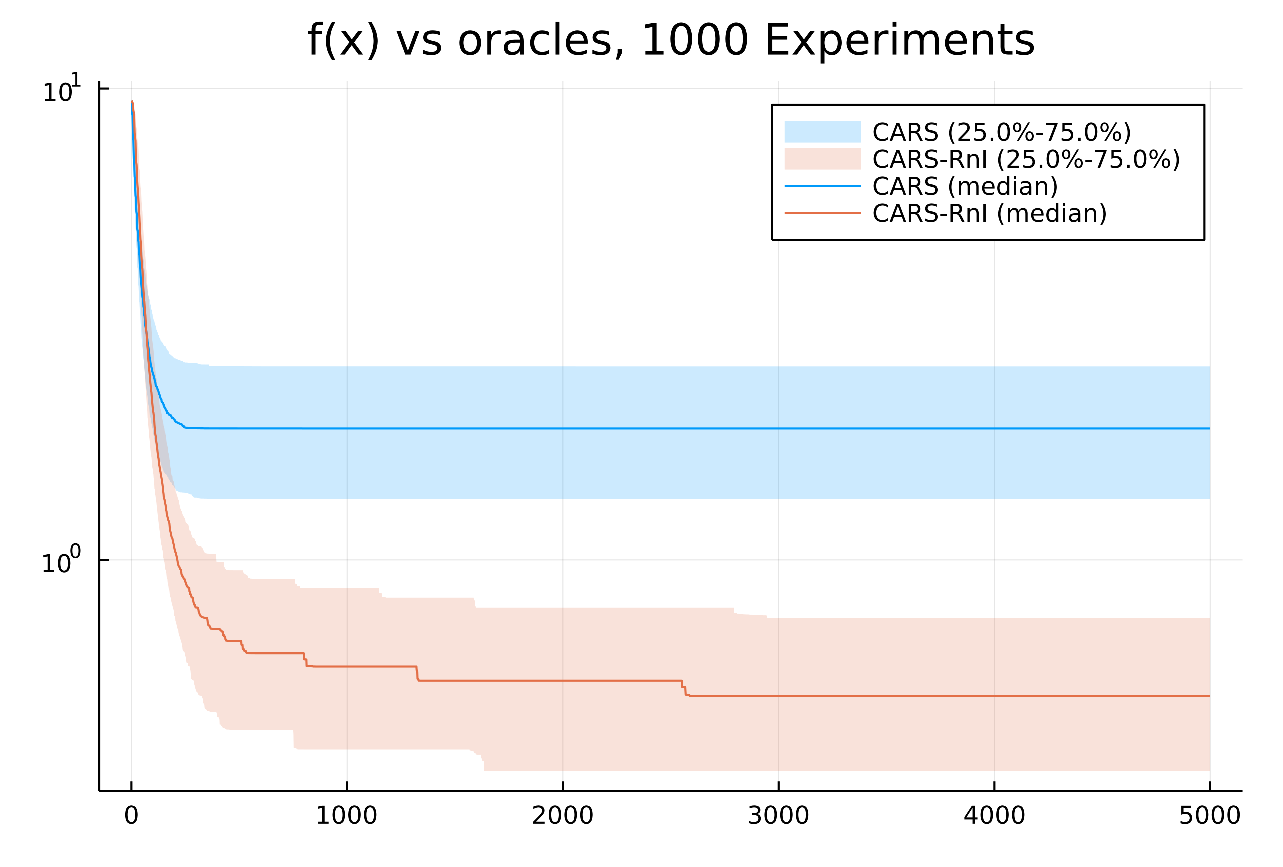
\includegraphics[width=0.7\linewidth]{freq10_amp0.2_quad_plus_sin.eps}}\\
    \vspace{3mm}
    {\includegraphics[width=0.7\linewidth]{freq10_amp0.2_quad_plus_sin_sols.eps}}
    \caption{Comparison of CARS and the Inspect-as-Running version of CARS for the quadratic function with sinusoidal noise.}
    \label{fig:Convex plus sine}
\end{figure*}
As depicted in Figure~\ref{fig:Convex plus sine}, the inspection strategy consistently identifies superior local minima, often reaching the global minima in a relatively lower dimension of 6.
We will revisit this example with a substantially higher dimension ($d=300$) for the comparison with global methods.

\subsection*{Ackley's Functions}
Ackley's functions are well-known non-convex functions with numerous spurious local minima:
\begin{equation*}
    f(x) = -20 \exp\left(-0.2 \sqrt{\|x\|^2/d}\right) - \exp\left(\sum_{i=1}^{d}{\cos(2\pi x_i)/d}\right) + e + 20.
\end{equation*}
 \cite{chen2019run} also introduced an asymmetric variant:
 \begin{align*}
    f(x,y) = -20 \exp(-0.04(x^2+y^2)) - \exp(0.7(\sin(xy) + \sin y) + 0.2\sin(x^2)) + 20
 \end{align*}
We tested both functions and again, observed that the IR version consistently found better minima, while the vanilla CARS frequently got trapped in a non-global local minima.
\begin{figure*}
    \centering
    {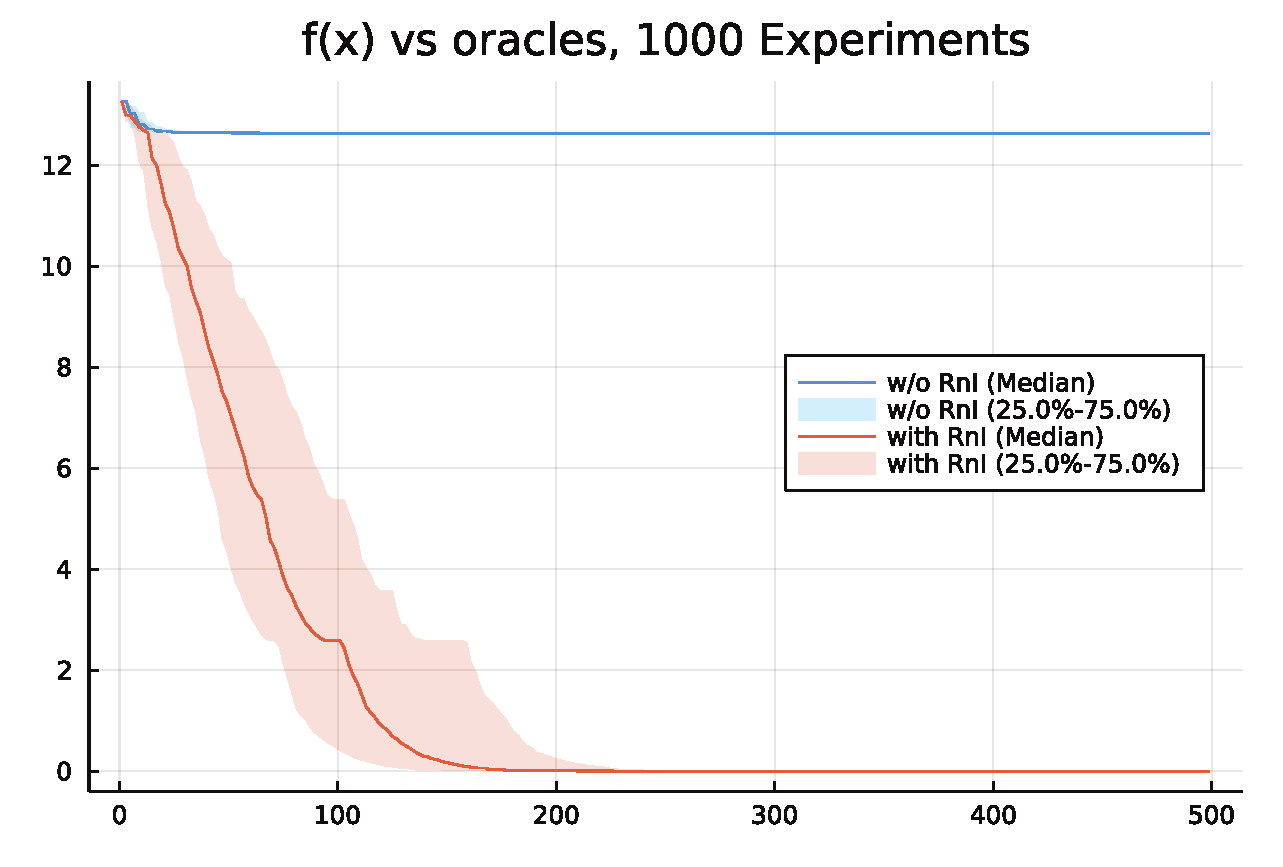
\includegraphics[width=0.7\linewidth]{Ackley.eps}}\\
    \vspace{3mm}
    {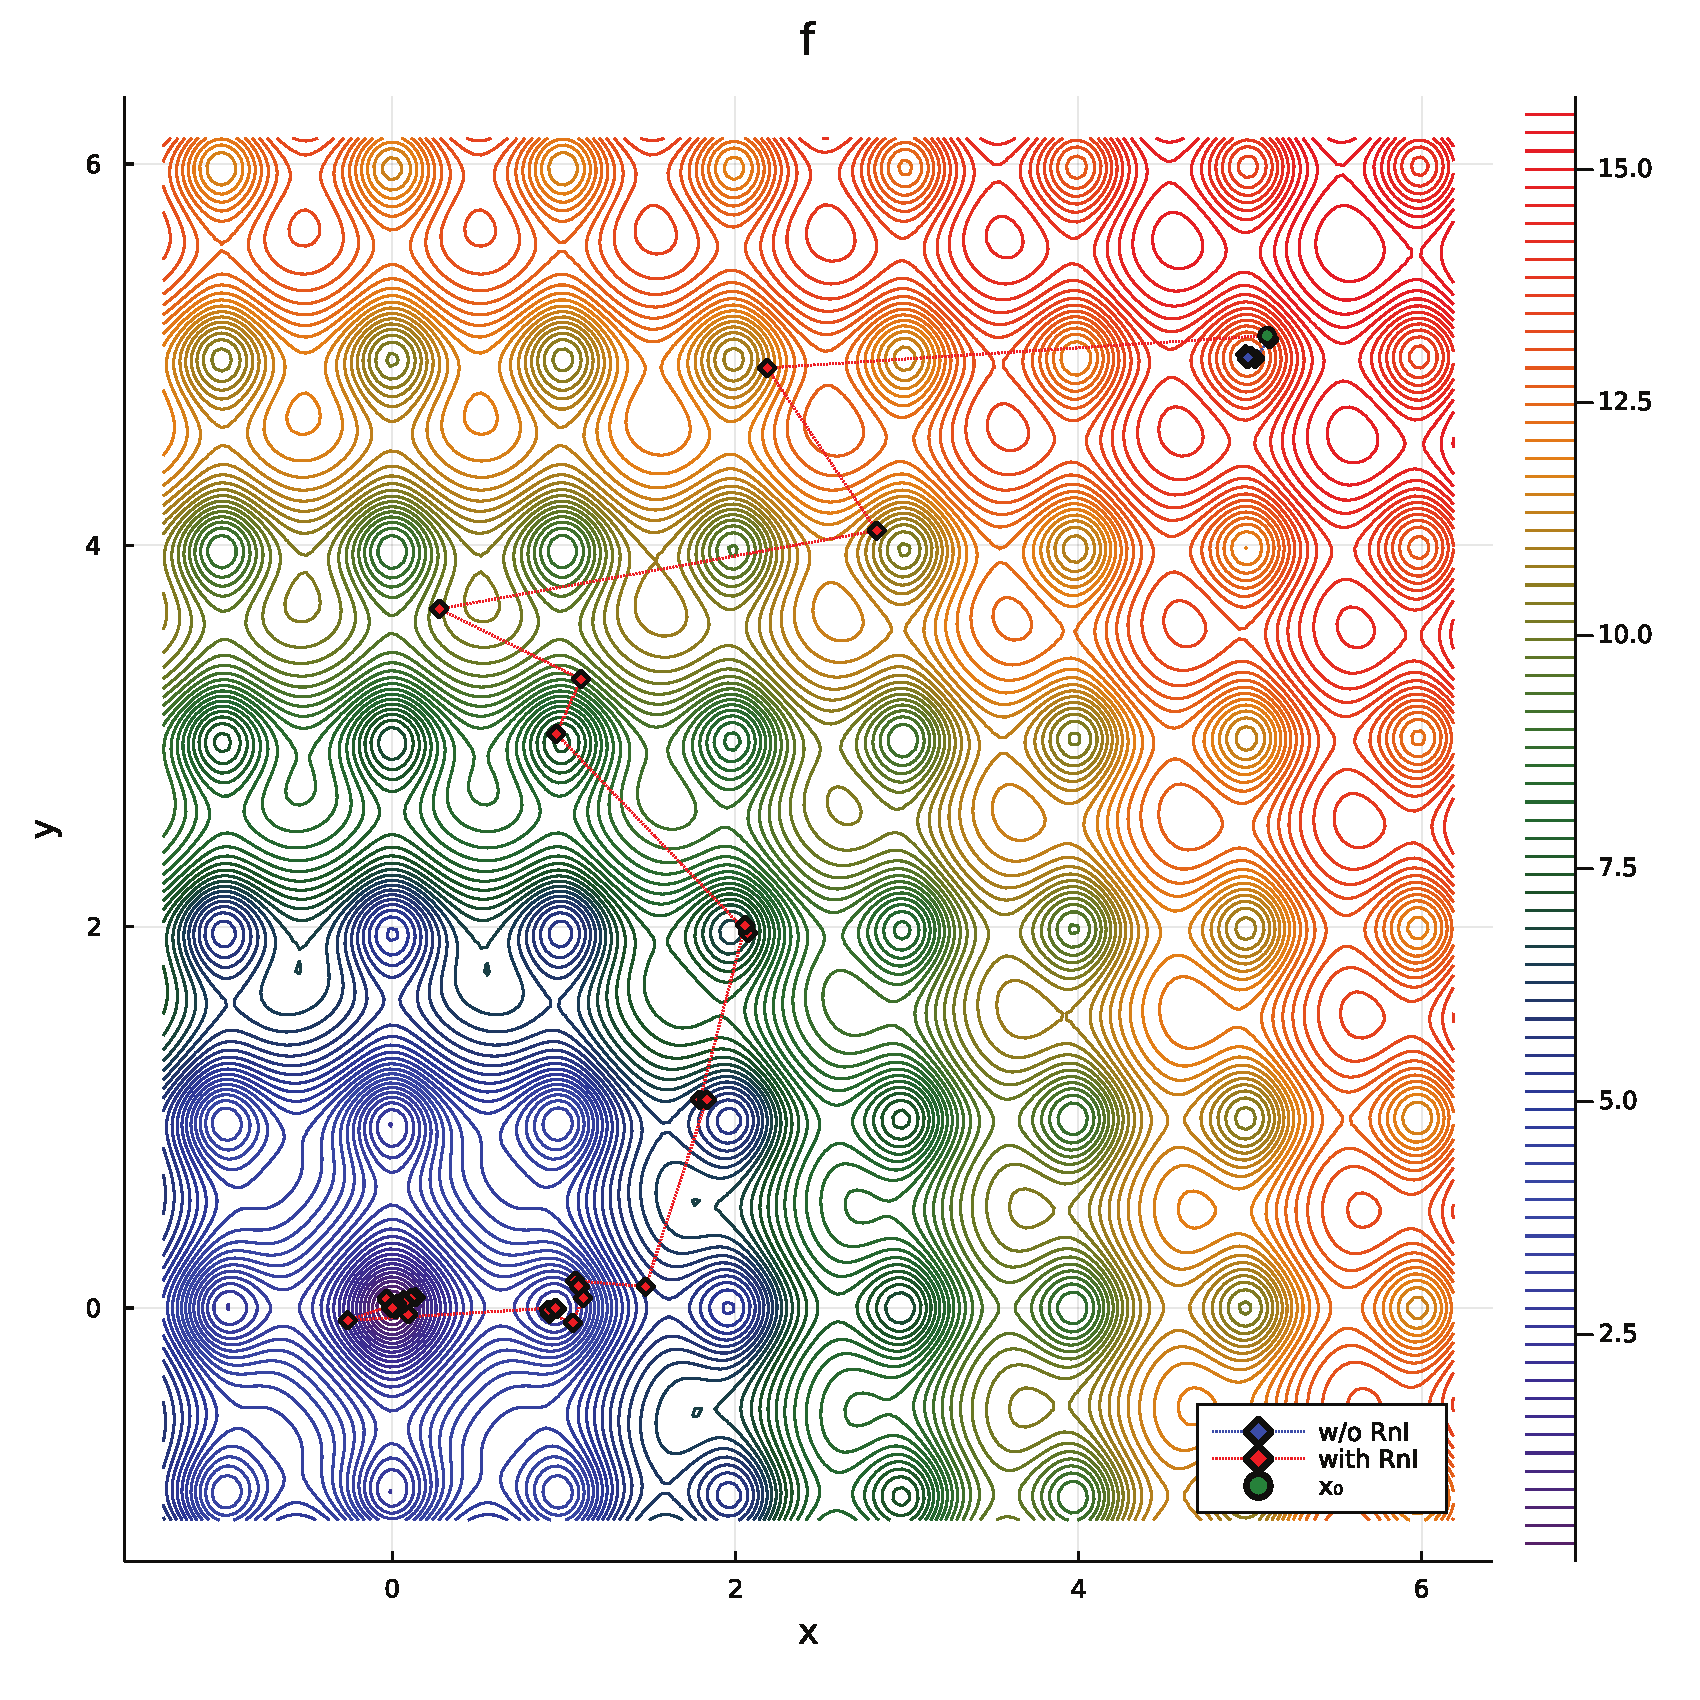
\includegraphics[width=0.7\linewidth]{Ackley_sols.eps}}
    \caption{Comparison of CARS and the Inspect-as-Running version of CARS for the Ackley function}
    \label{fig: Ackley}
\end{figure*}

\begin{figure*}
    \centering
    {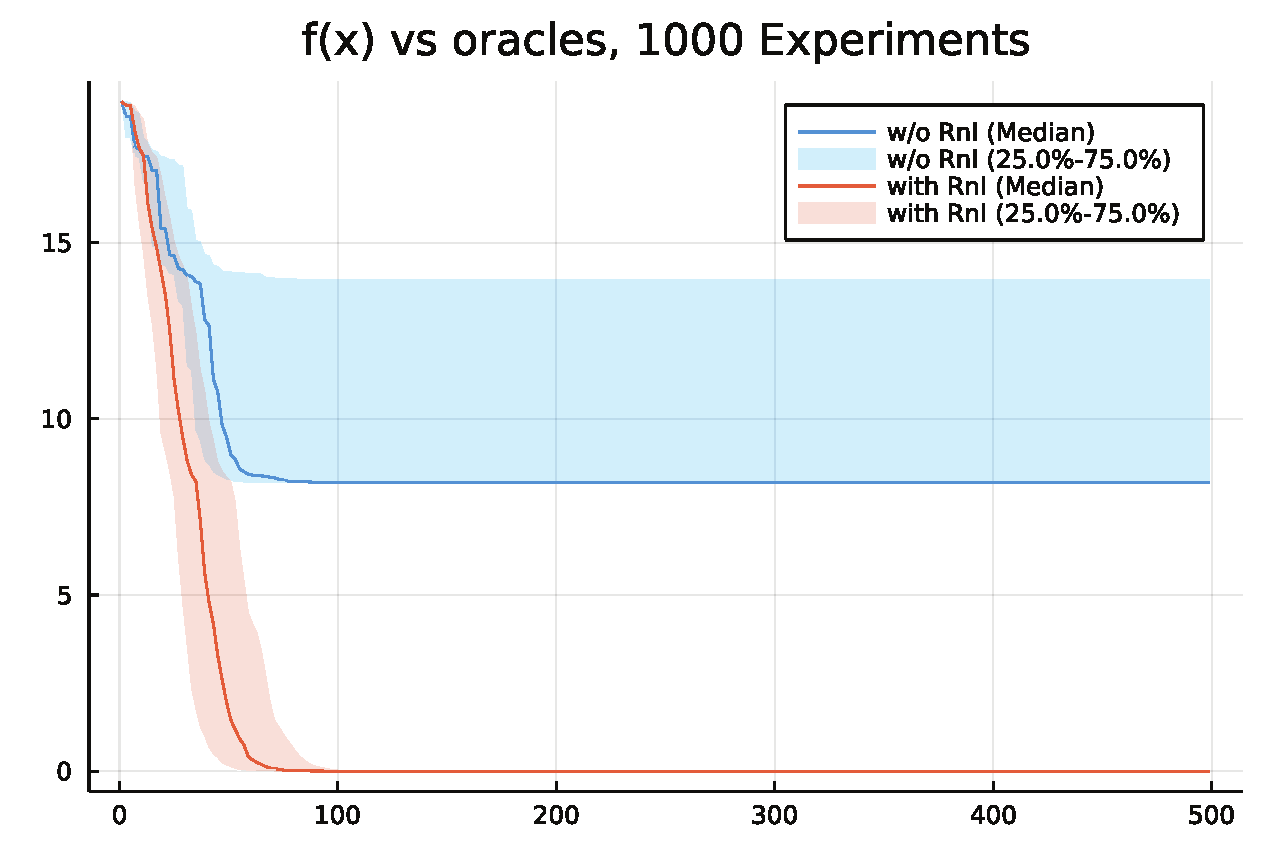
\includegraphics[width=0.7\linewidth]{asym_Ackley.eps}}\\
    \vspace{3mm}
    {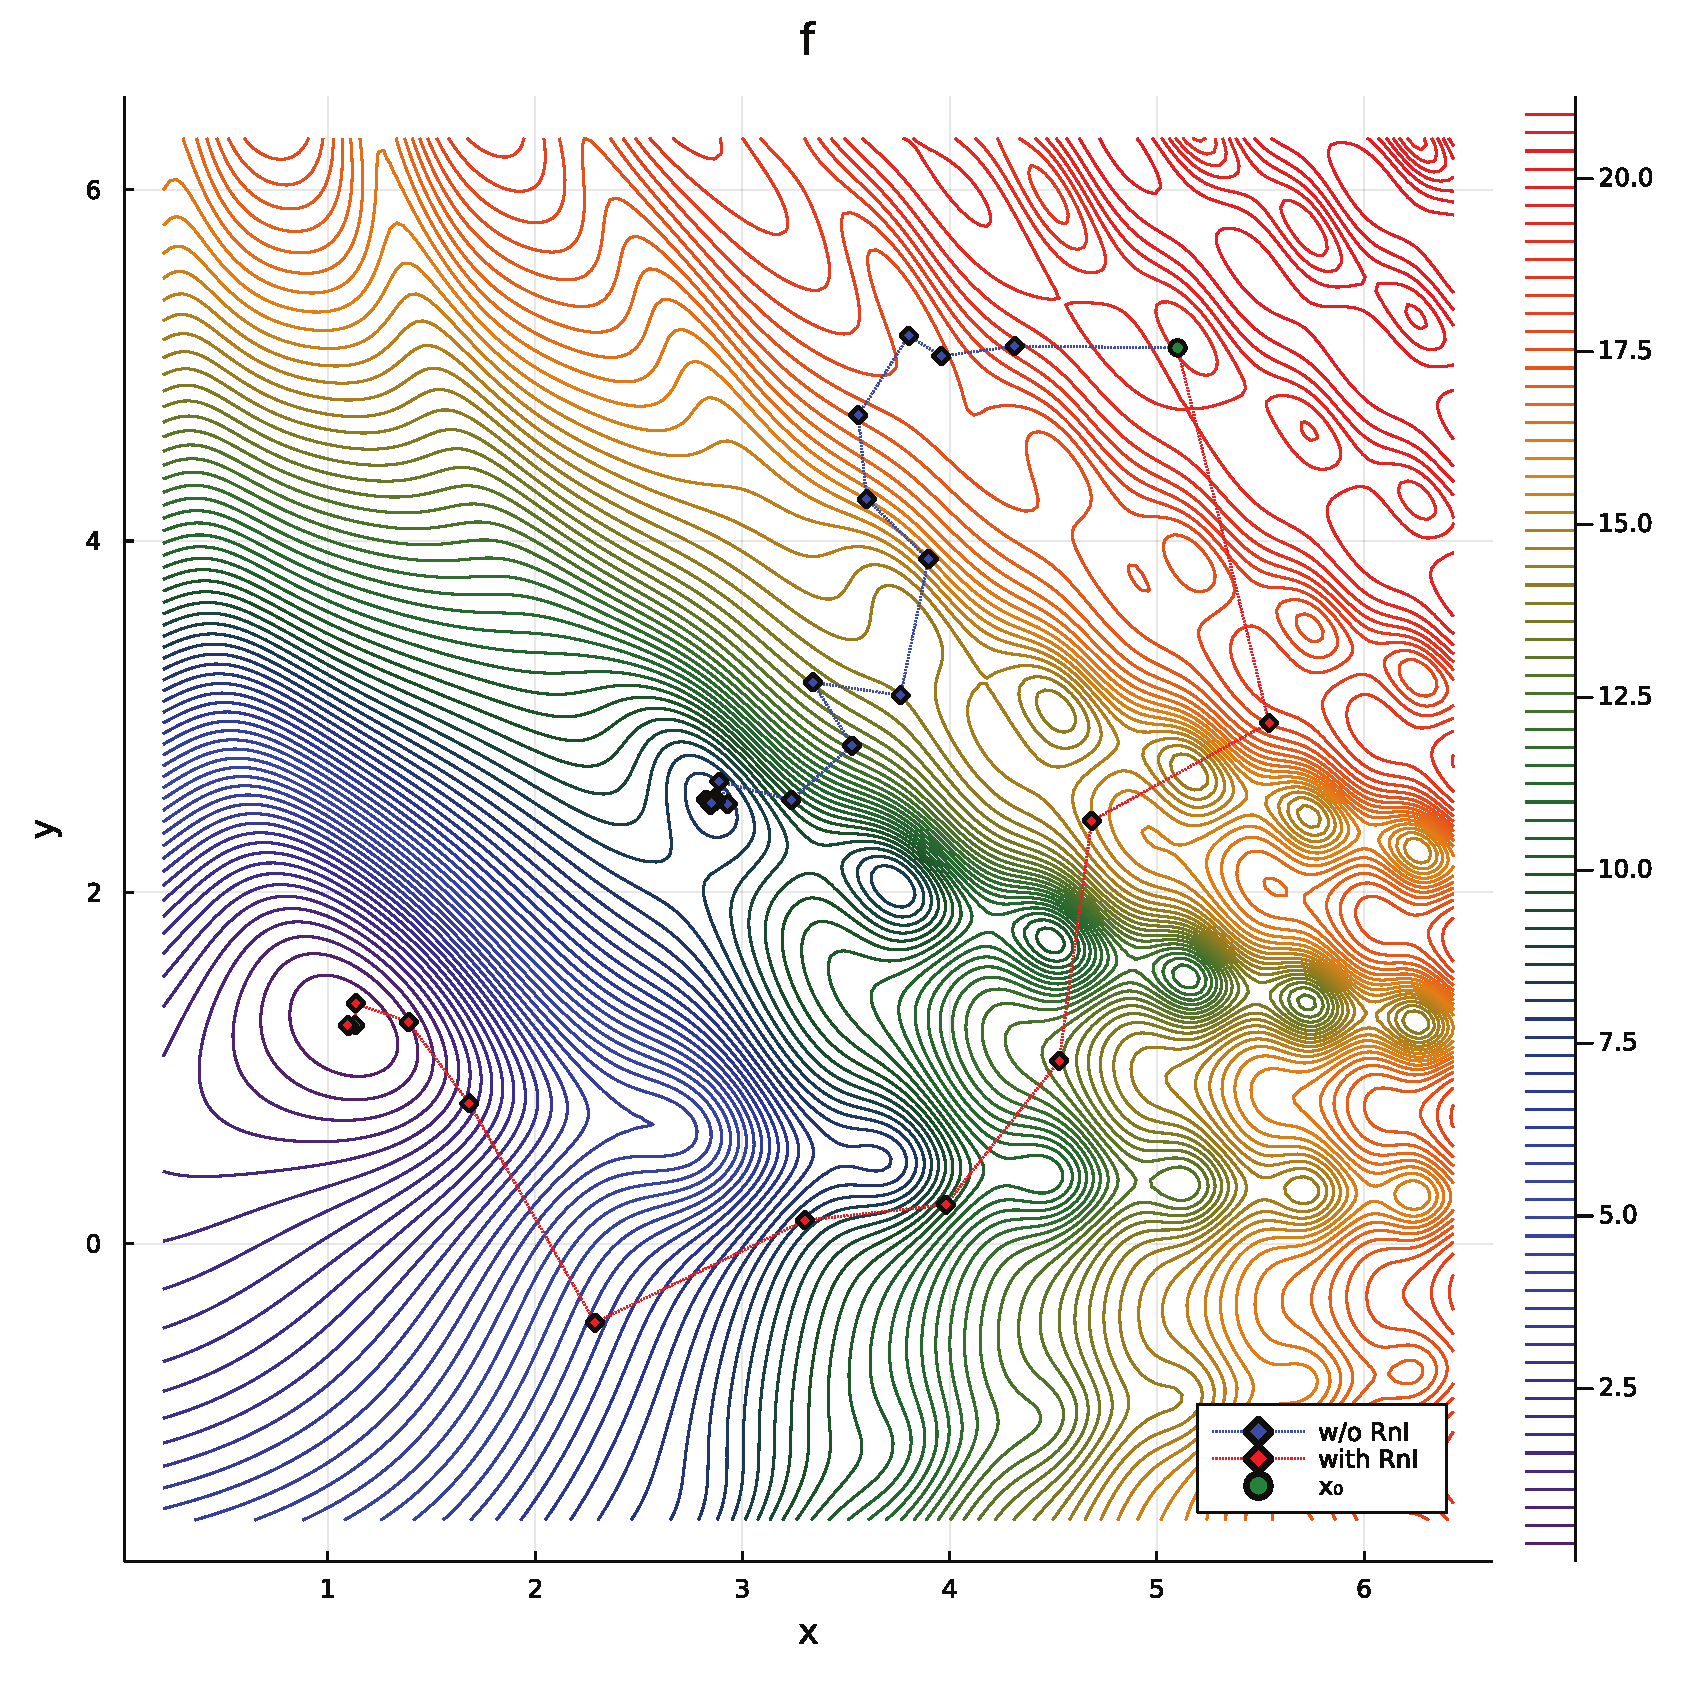
\includegraphics[width=0.7\linewidth]{asym_Ackley_sols.eps}}
    \caption{Comparison of CARS and the Inspect-as-Running version of CARS for the asymmetric Ackley function}
    \label{fig: Ackley asymmetric}
\end{figure*}

\subsection*{K-means Clustering}
Let $\{x_i\}_{i=1}^{n}$ be a set of $n$ points in $\mathbb{R}^d$ and $\{z_j\}_{j=1}^{K}$ be $K$ points in $\mathbb{R}^d$. Let the variable $Z = [z_1, \cdots, z_K] \in \mathbb{R}^{d \times K}$ be the matrix of the cluster centers. The K-means clustering problem is to find the optimal $Z$ that minimizes the following objective function:
\begin{equation*}
    f(Z) = \frac{1}{2n} \sum_{i=1}^{n} \min_{j=1,\cdots,K} \|x_i - z_j\|^2.
\end{equation*}
We tackle this problem with derivative-free methods by treating $Z$ as a vector in $\mathbb{R}^{dK}$.

\subsubsection*{Synthetic Gaussian data from \cite{yin2018stochastic}}
The first problem has synthetic Gaussian data, which is a mixture of four multivariate Gaussian distributions with $n = 1000$ each. This problem is introduced in \cite{yin2018stochastic}. We used the same means and covariance matrices:
\begin{align*}
    \mu_1 = [-5, -3], \mu_2 = [5, -3], \mu_3 = [0, 5], \mu_4 = [2.5, 4],
\end{align*}
    and 
\begin{align*}
    \Sigma_1 = \begin{bmatrix}
        0.8 & 0.1 \\ 0.1 & 0.8
    \end{bmatrix}, 
    \Sigma_2 = \begin{bmatrix}
        1.2 & 0.6 \\ 0.6 & 0.7
    \end{bmatrix}, 
    \Sigma_3 = \begin{bmatrix}
        0.5 & 0.05 \\ 0.05 && 1.6
    \end{bmatrix},
    \Sigma_4 = \begin{bmatrix}
        1.5 & 0.05 \\ 0.05 & 0.6
    \end{bmatrix}.
\end{align*}
\begin{figure*}
    \centering
    {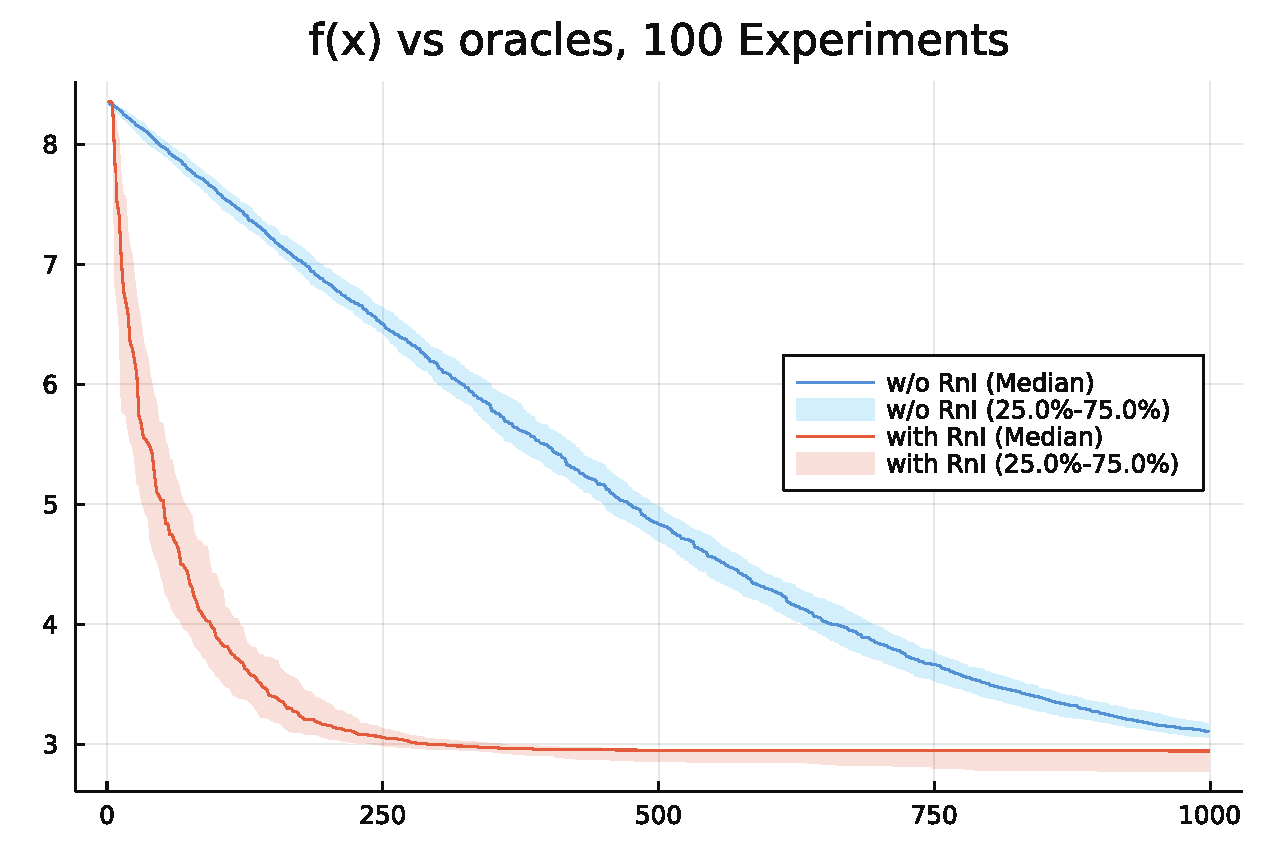
\includegraphics[width=0.7\linewidth]{Kmeans_h0_0.136.eps}}\\
    \vspace{3mm}
    {\includegraphics[width=0.7\linewidth]{Kmeans_h0_0.136_2dplot.eps}}
    \caption{Comparison of CARS and the Inspect-as-Running version of CARS for the K-means clustering problem of synthetic Gaussian data}
    \label{fig: K-means synthetic}
\end{figure*}

\subsubsection*{Iris data}
The second K-means clustering problem consists of the Iris dataset. This dataset contains 150 samples of three different species of Iris flowers. Each sample has four features: sepal length, sepal width, petal length, and petal width.
\begin{figure}
    \centering
    {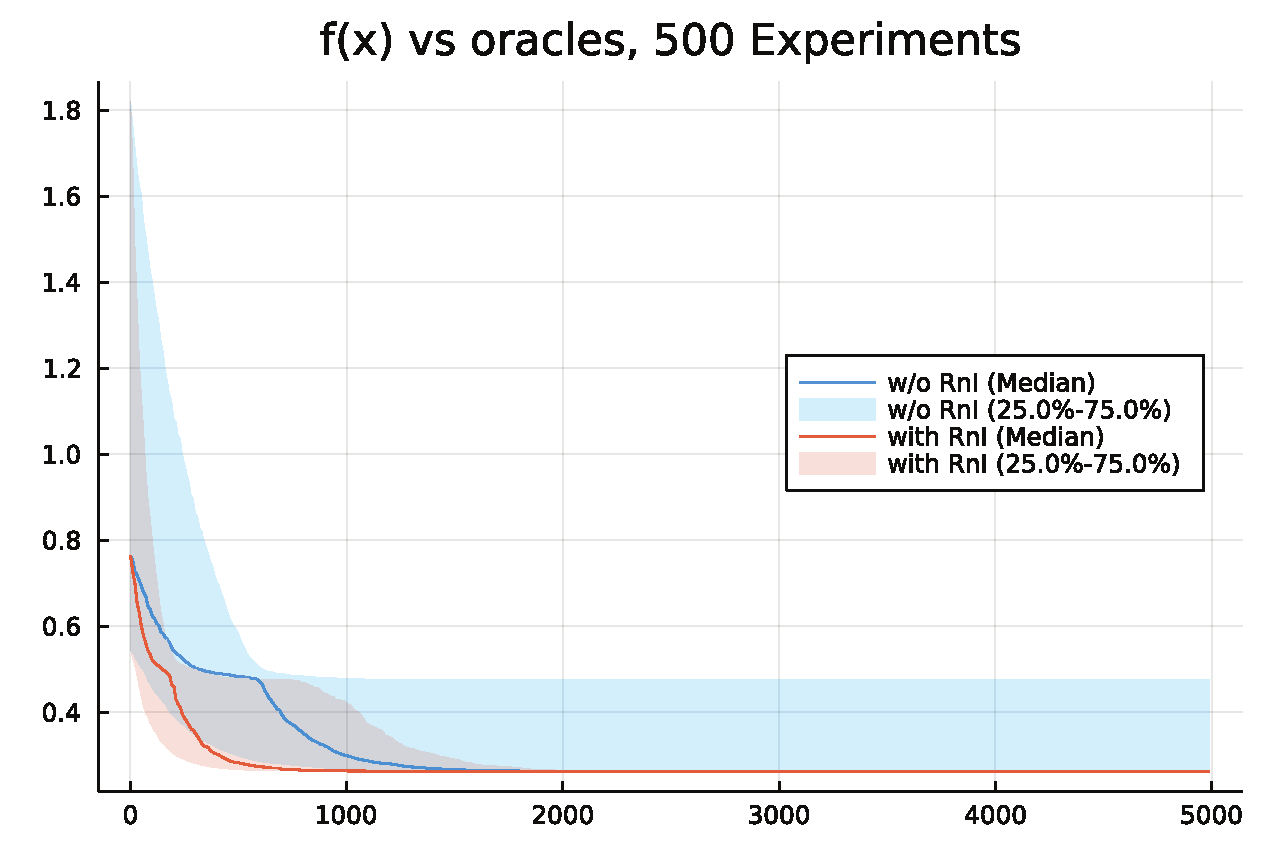
\includegraphics[width=0.7\linewidth]{Iris_h0_1.36e-3_R3.eps}}\\
    \vspace{3mm}
    {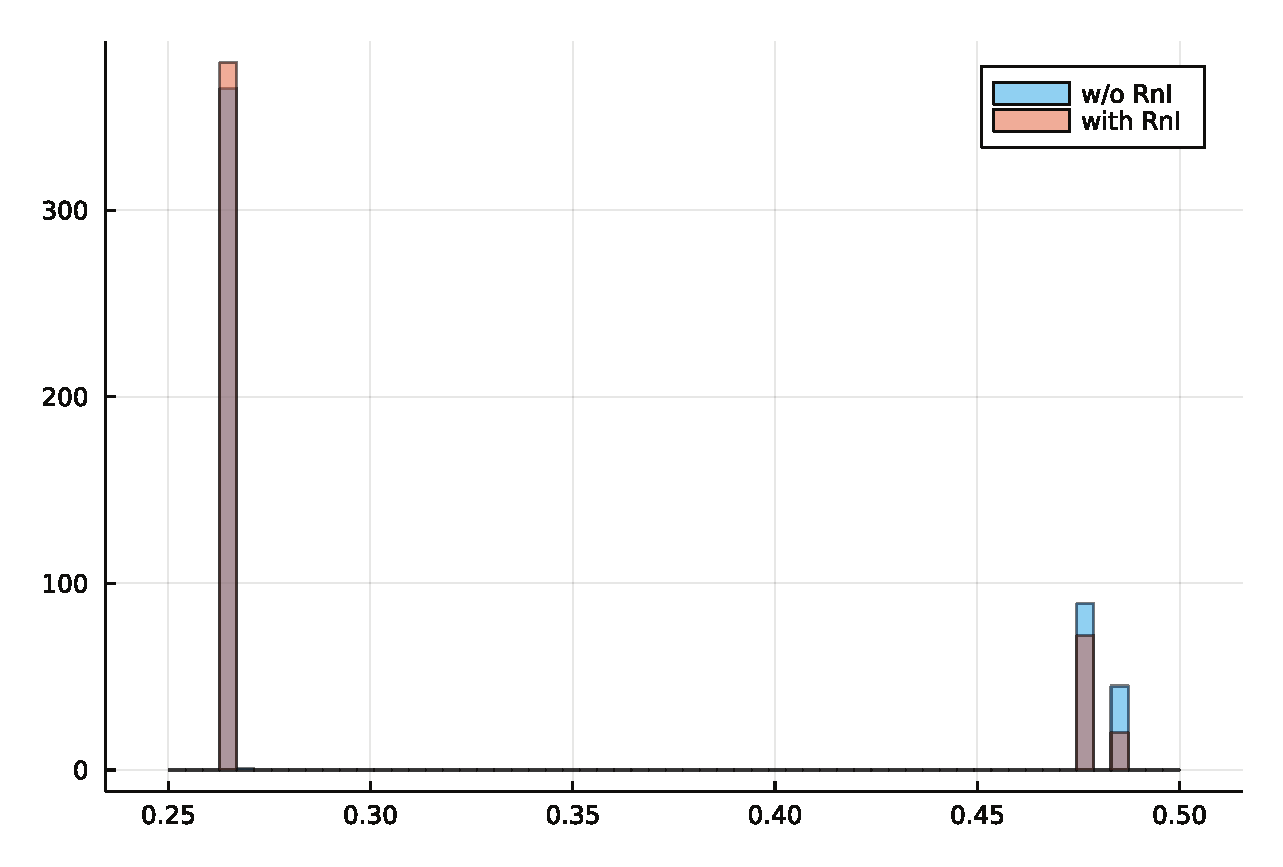
\includegraphics[width=0.7\linewidth]{Iris_histogram.eps}}
    \caption{Comparison of CARS and the Inspect-as-Running version of CARS for the K-means clustering of the Iris dataset}
    \label{fig: K-means Iris}
\end{figure}
We illustrate the results from 500 runs and the histogram of the final objective values in Figure~\ref{fig: K-means Iris}.
The figures demonstrate that the IR version of CARS finds better minima in most cases, and more rapidly.

\subsection*{Hyperparameter tuning}
We applied the two versions of CARS to hyperparameter tuning for training a convolutional neural network on the MNIST dataset.
The hyperparameters included the $L^2$ regularization parameter in the loss, the learning rate for the optimizer (AdaDelta), and the annealing rate for the scheduler (StepLR). To show the ability to escape the local minima more clearly, we started from a suboptimal initial point $x_0 = (0.5, 0.5, 0.5)$.

To reduce the variance, the objective function for the hyperparameter is set to be the mean of two samples, which measures the misclassification rate of the trained model with the given set of hyperparameters.

\begin{figure}
    \centering
    {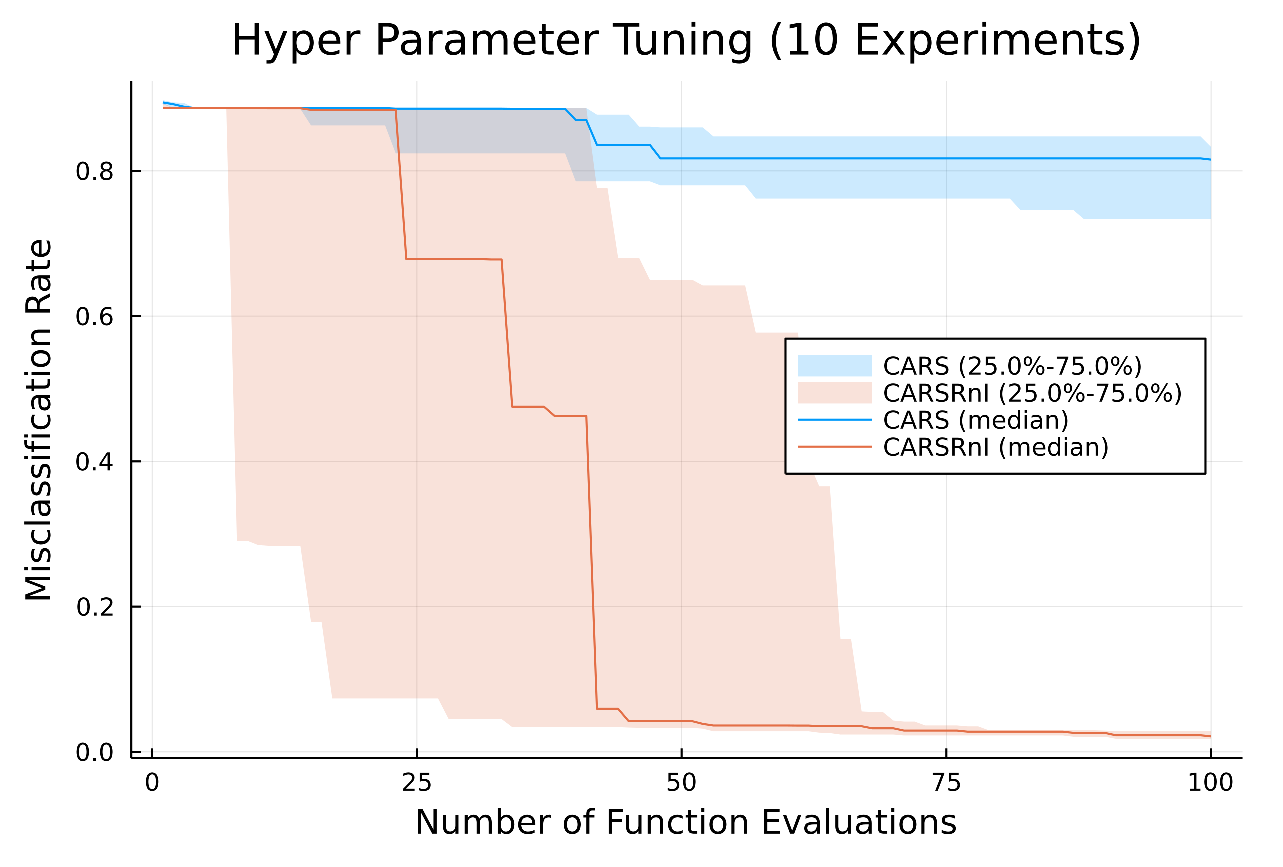
\includegraphics[width=0.7\linewidth]{CARS_vs_CARSRnI_julia.eps}}\\
    \vspace{3mm}
    {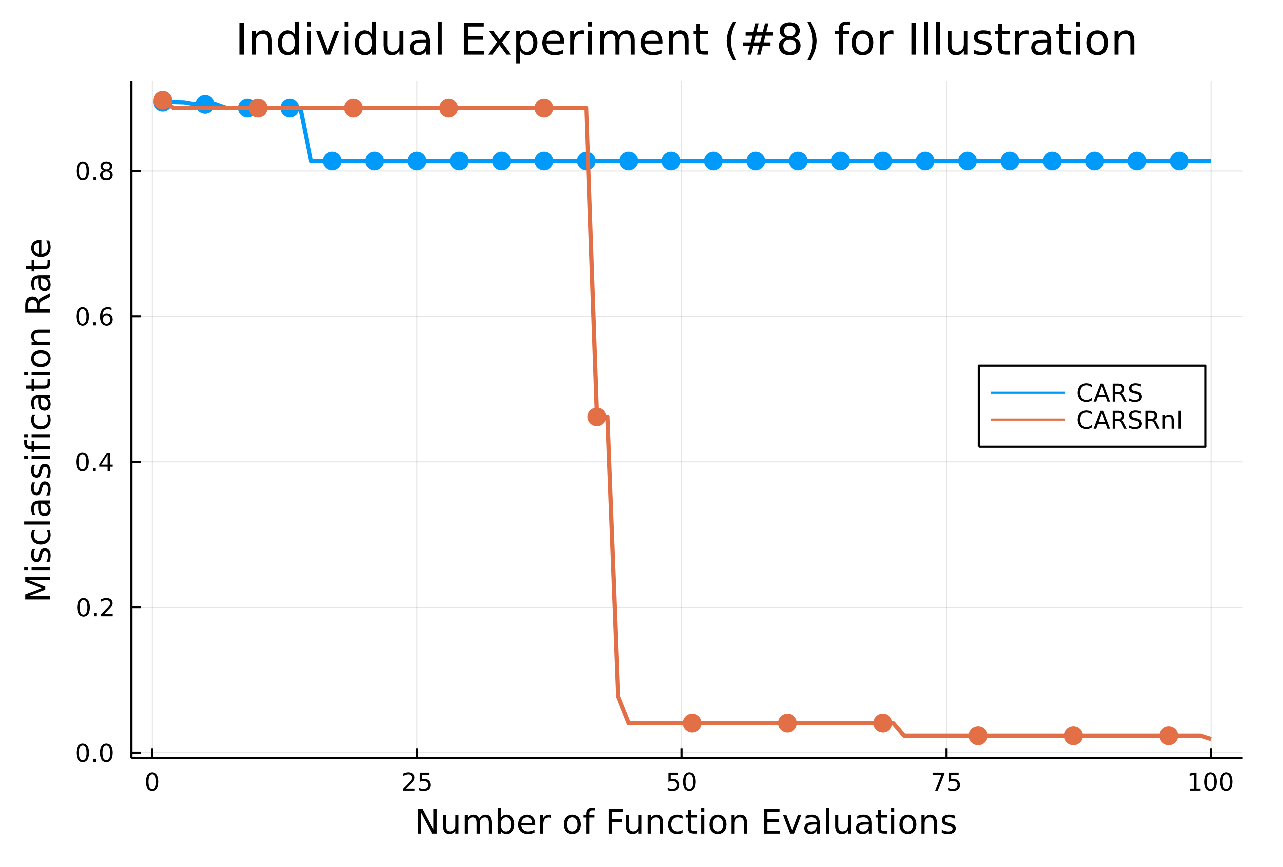
\includegraphics[width=0.7\linewidth]{CARS_vs_CARSRnI_Individual_julia.eps}}
    \caption{Comparison of CARS and the Inspect-as-Running version of CARS for hyperparameter tuning for training a convolutional neural network for MNIST dataset}
    \label{fig: HP Tuning - MNIST}
\end{figure}

\subsection*{Spurious local minima in higher dimension}
We revisit the function with spurious local minima in higher dimension, $d=300$, and compare the performance of CARS and the IR version of CARS with the global method RBFOpt \cite{costa2018rbfopt}, which is one of the most efficient the global methods.
RBFOpt took 15,073 seconds for 1,000 iterations (1,241 function evaluations), while CARS ran in 1.474 seconds for 30,000 function evaluations.
Here we see that the computational cost of the solver itself (sub-problems) is much higher in the global methods, often making it impractical for high-dimensional problems.
Furthermore, to utilize the structure of the problem, namely independence of each variable, we adopted the coordinate descent version, by simply replacing the sampling directions from $\unif(\mathbb{S}^{d-1})$ to $\unif(\{e_1, \cdots, e_d\})$, both for CARS and inspections.
\begin{figure}
    \centering
    {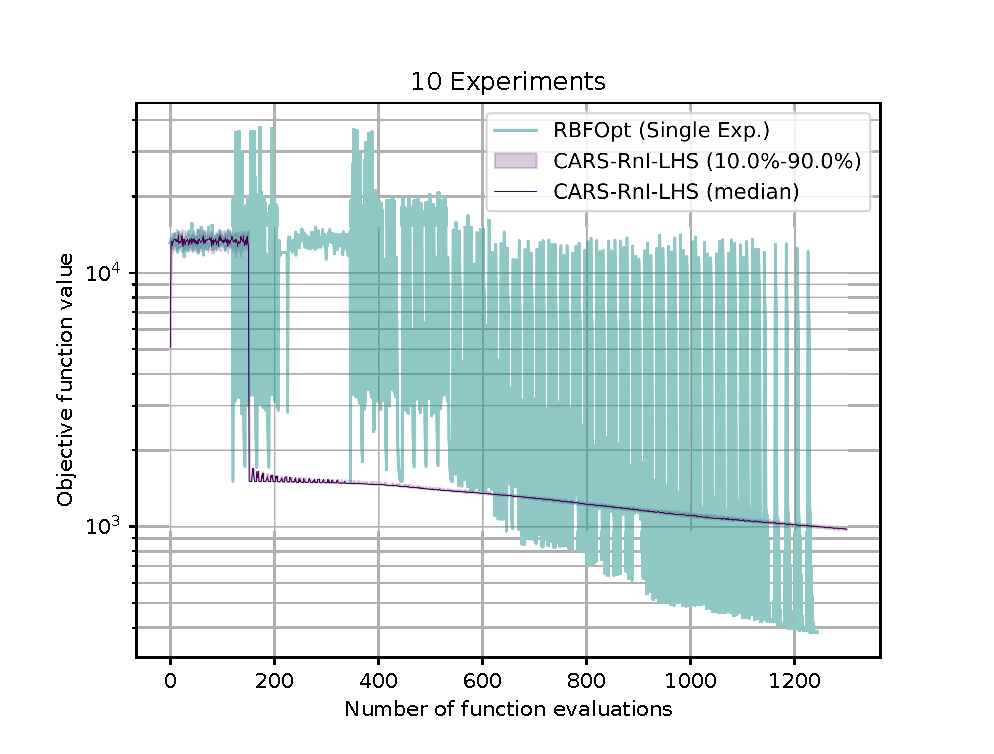
\includegraphics[width=0.7\linewidth]{X_small_300dim.eps}} \\
    \vspace{3mm}
    {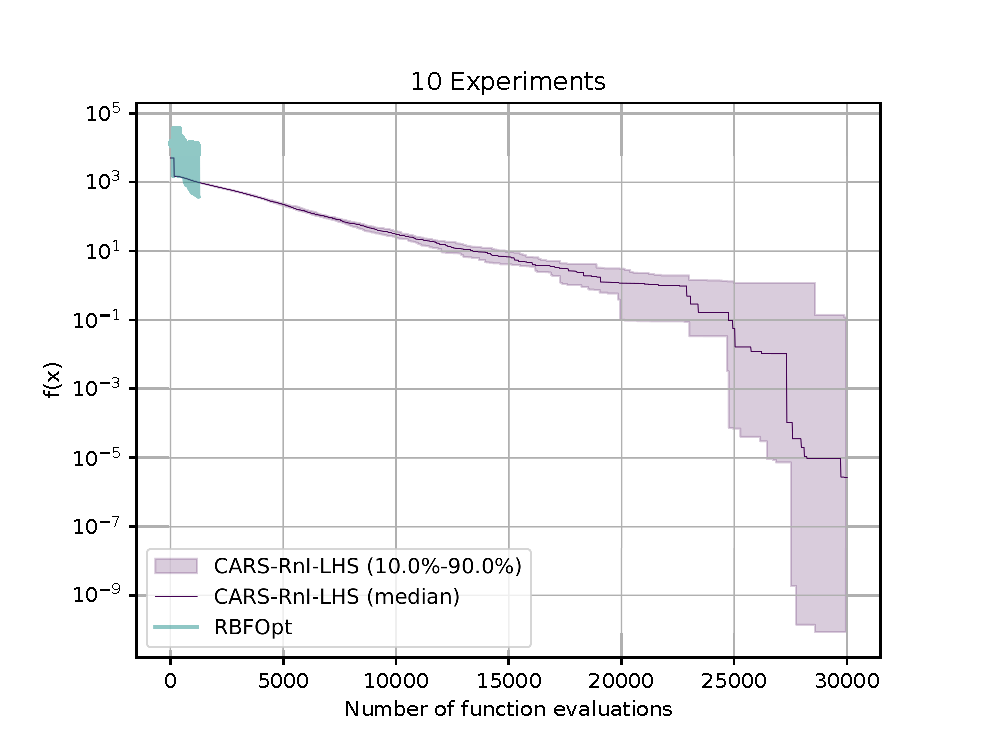
\includegraphics[width=0.7\linewidth]{X_all_300dim.eps}}
    \caption{Comparison of CARS with IR and the RBFOpt in 300-dimensional problem with spurious local minima. Computation for RBFOpt is terminated after 1,000 iterations due to the computational cost.}
\end{figure}
